% A good introduction to latex can be found here:
%    http://www.cse.ohio-state.edu/~hank/latex/lshort141.pdf

\documentclass[9.5pt]{extarticle}

\usepackage{full page}  % make the margins somewhat smaller than the default
\usepackage{graphicx}
\usepackage{amsmath}
\usepackage{indentfirst}
\usepackage{color}
\usepackage{cite}
\usepackage{wasysym}
\usepackage{amssymb}
\usepackage{multirow}
\usepackage{float}
\usepackage{lscape}
\usepackage{alltt} 
\usepackage{listings}
\usepackage{booktabs}
\usepackage{mathtools}
\usepackage{fancyhdr}

\DeclarePairedDelimiter{\ceil}{\lceil}{\rceil}
\DeclarePairedDelimiter{\floor}{\lfloor}{\rfloor}

\definecolor{dkgreen}{rgb}{0,0.6,0}
\definecolor{gray}{rgb}{0.5,0.5,0.5}
\definecolor{mauve}{rgb}{0.58,0,0.82}

\lstset{frame=tb,
  language=matlab,
  aboveskip=3mm,
  belowskip=3mm,
  showstringspaces=false,
  columns=flexible,
  basicstyle={\small\ttfamily},
  numbers=none,
  numberstyle=\tiny\color{gray},
  keywordstyle=\color{blue},
  commentstyle=\color{dkgreen},
  stringstyle=\color{mauve},
  breaklines=true,
  breakatwhitespace=true
  tabsize=3
}



\usepackage{listings}  %  needed for source code listings
\lstset{language=Java}         

% set the document title, author, and date here.
%  once set, the \maketitle command (within the document)
%  will display them nicely
\title{Missionaries and Cannibals}
\author{Chua Zheng Fu Edrei}

\begin{document}
\maketitle

\section{Introduction}

Three missionaries, three cannibals and a boat is at one side of the river and would like to cross to the other side. There are two constraints: (1) the boat can carry one or two people at a time; and (2) at any time there must be at least as many missionaries as cannibals on either side of the river.

\begin{figure}[H]
\centering
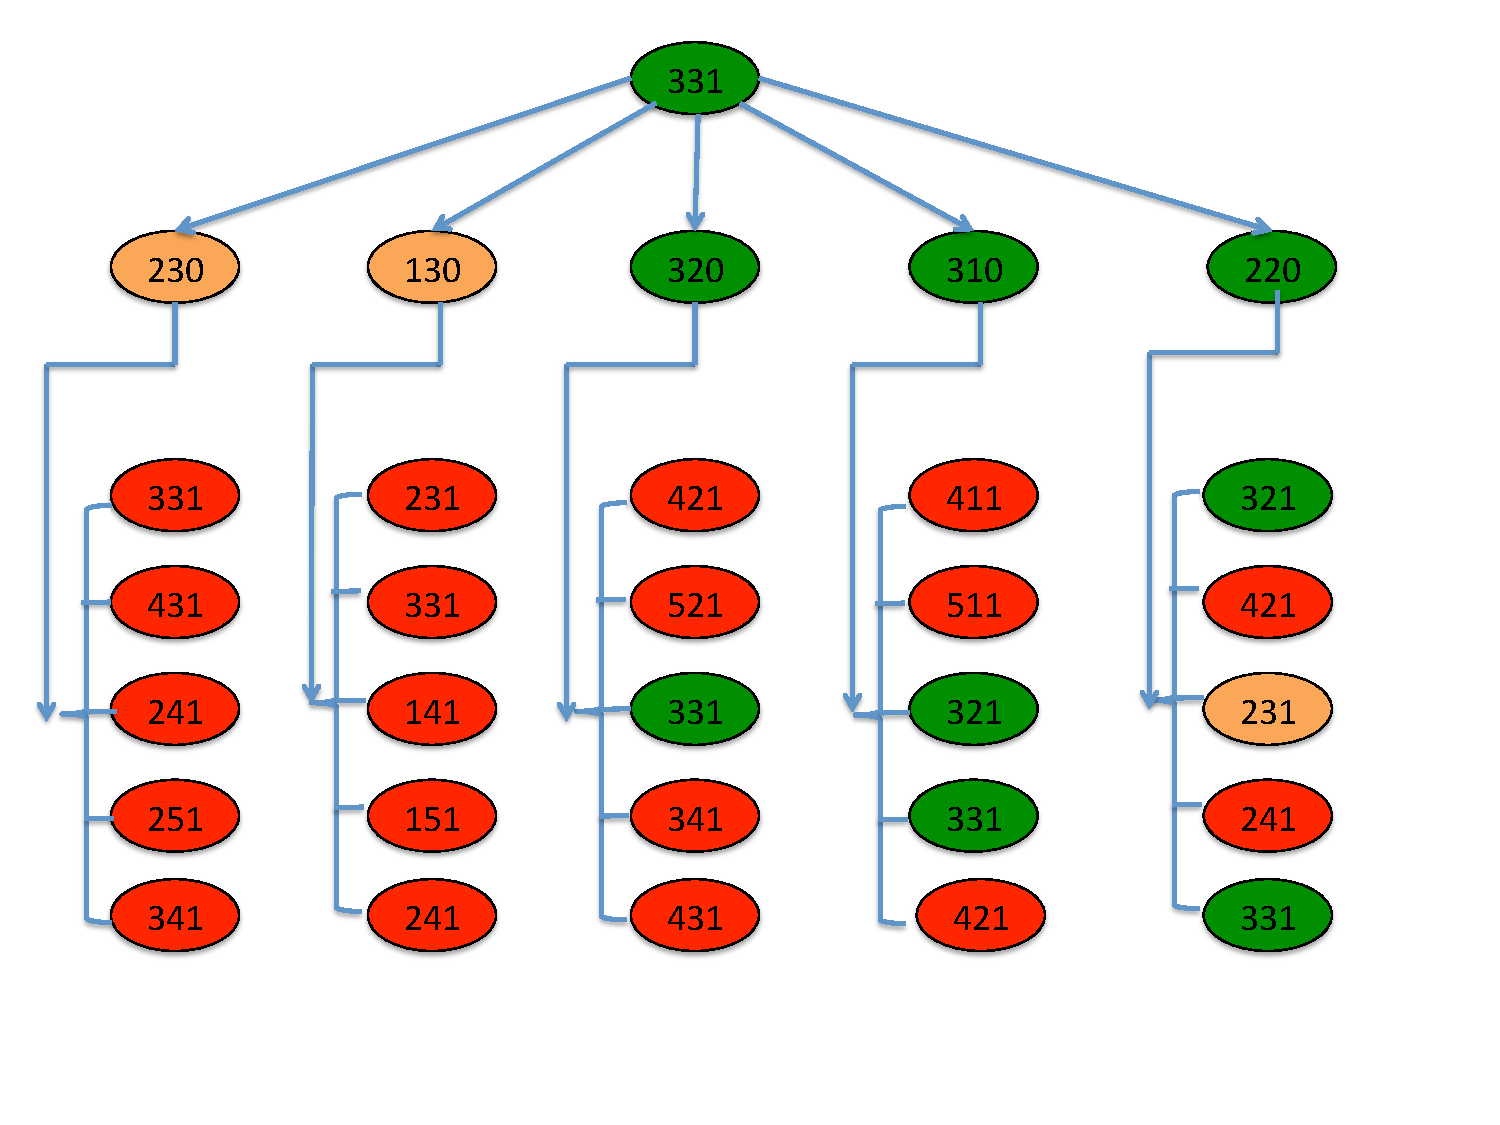
\includegraphics[scale=0.4]{stategraph.pdf}
\caption{Graph of states: Green denotes legal states, Orange and Red denote illegal states. Orange is illegal because it represents a state in which missionaries will be eaten by cannibals and Red is illegal because the state is unattainable (previous state is illegal or it represents more people than the total number of people originally) }
\label{Figure 1}
\end{figure}

We can represent the state of the system using the notation $(m,c,b)$, where $m$ is the number of missionaries at the starting bank, $c$ is the number of cannibals at the starting bank and $b$ is the number of boat at the starting bank. If the total number of missionaries is $T_m$, the total number of cannibals is $T_c$ and the total number of boats is $T_b$, we can represent the other bank using $(T_m-c,T_c-c, T_b-b)$ and therefore, the three numbers are adequate to represent the state of the whole system.\\

In the given problem, $T_m=3$, $T_c=c$ and $T_b=1$ and the goal is to transit from the start state $(3,3,1)$ to the goal state $(0,0,0)$. We can calculate an upper bound to the number of state for this specific question by considering that $0\le m \le 3$, $0 \le c \le 3$ and $0 \le b \le 1$. Therefore, if we ignore illegal states, the upper bound on the number of states for this specific problem is given as $S \le 4 \times 4 \times 2$ or $S \le 32$. We can generalize this statement for any problem to be $ S  \le (T_m+1) \times (T_c+1) \times (T_b + 1)$.\\

Figure 1 shows a graph of the states for the first three level. When the boat is at the starting bank, the next action will bring the boat to the finishing bank and there are five possibilities: a missionary cross the river, two missionaries cross the river, a cannibal cross the river, two cannibals cross the river, and one missionary with one cannibal cross the river. Green states in the graph denotes legal state. Orange and  Red denote illegal states. Orange is illegal because it represents a state in which missionaries will be eaten by cannibals (i.e. $c>m$ when $m \neq 0$ or $T_c - c > T_m - m$ when $T_m - m \neq 0$). Red is illegal because the state is unattainable (either previous state is illegal or it represents more people than the total number of people originally).


\section{Implementation of the model}

The model is implemented in \verb`CannibalProblem.java`.  Here's my code for \verb`getSuccessors`:

\begin{lstlisting}[language=java,caption={Java code for getSuccessors}]
public ArrayList<UUSearchNode> getSuccessors() {
	 ...
	int b = state[2] == 0 ? 1 : 0; // change the boat state
	// loop through all possible combination of movement of missionaries and cannibals
	for(int moveMissionaries = 0; moveMissionaries <= BOAT_SIZE; moveMissionaries++){
		for(int moveCannibals = 0; moveCannibals <= BOAT_SIZE - moveMissionaries; moveCannibals++) {
			if(state[2] == 1) { // move away from start bank
				numMissionaries = state[0] - moveMissionaries;
				numCannibals = state[1] - moveCannibals;
			}else{ // move towards the finish bank
				numMissionaries = state[0] + moveMissionaries;
				numCannibals = state[1] + moveCannibals;
			}
			CannibalNode potentialSuccessor = new CannibalNode(numMissionaries,numCannibals,b,depth);

			// check if there is >= 1 person on boat and successor is legal and safe 
			if(moveCannibals+moveMissionaries != 0 && potentialSuccessor.isLegalState()
				&& potentialSuccessor.isSafeState()){
				array.add(potentialSuccessor);
			}
		}
	}
	return array;
}
\end{lstlisting}

The basic idea of \verb`getSuccessors` is to attempt all 5 possible combinations that a state can change into based on the five possibilities discussed above. If the boat is at the start bank, we can move the missionaries and/or the cannibals to the finishing bank and vice versa. Finally, we check for legal and safe states from the combination of next states that are produced.\\

I used a method \verb`isSafeState` that returns \verb`true` if the state does not result in more cannibals than missionaries on either side of the bank i.e. $c\leq m$ when $m \neq 0$ or $T_c - c \leq T_m - m$ when $T_m - m \neq 0$. I also used a method \verb`isLegalState` that returns \verb`true` if $c < 0$ or $ m < 0$ or $c > totalCannibals$ or $m > totalMissionaries$.\\

I tested my code by including a  \verb`main` method as shown in listing 1 and getting the successors for states $(3,3,1)$, $(3,2,0)$, $(3,1,0)$ and $(2,2,0)$. I verified that the successors are correct by comparing the generated results with the graph that is obtained manually in Figure 1.

\begin{lstlisting}[language=java,caption={Java code for testing}]
public static void main(String args[]){

	CannibalNode startnode = new CannibalNode(3,3,1,0);
	ArrayList<CannibalNode> list = startnode.getSuccessors();

	for(CannibalNode i : list) 
		System.out.println(i.toString());
}
\end{lstlisting}

\section{Breadth-first search}

\begin{lstlisting}[language=java,caption={Java code for BFS}]
public List<UUSearchNode> breadthFirstSearch(){

	LinkedList<UUSearchNode> frontier = new LinkedList<>(); // queue
	HashSet<UUSearchNode> visited = new HashSet<>(); // the visited states
	HashMap<UUSearchNode,UUSearchNode> backchainMap = new HashMap<>(); // backchaining map
	frontier.addLast(startNode); // add the starting node
	visited.add(startNode);
	incrementNodeCount();

	while(!frontier.isEmpty()) { // classic BFS
		updateMemory(visited.size()); // Update memory
		UUSearchNode tovisit = frontier.removeFirst(); // visit node from frontier
		if (tovisit.goalTest()) //termination condition
			return backchain(tovisit, backchainMap);
		for (UUSearchNode child : tovisit.getSuccessors()) {
			if(!visited.contains(child)) {
				backchainMap.put(child, tovisit);
				frontier.addLast(child); // add to linked list
				visited.add(child);
			}
		}
		return null;
	}
}
\end{lstlisting}

I implemented a classic breadth-first search, using a hash table to keep track of the visited states. A hash table is an ideal data structure to track the visited state because it has constant $\theta(1)$ retrieval time, compared to a linked list which will have linear $O(n)$ retrieval time.\\

A linked list, which acts as a queue, is used to keep track of the next states to visit in order to ensure that the search proceeds in increasing order of depth (characteristic of BFS). The code for  \verb`breadthFirstSearch` is presented in Listing 3. I also used backchaining to extract the path from the goal state back to the start state and the code for \verb`backchain` is presented in Listing 4. Basically, it uses the reference stored in the HashMap to back trace from one state to the previous state.\\

\begin{lstlisting}[language=java,caption={Java code for backchaining}]
private List<UUSearchNode> backchain(UUSearchNode node, HashMap<UUSearchNode, UUSearchNode> visited) {
	LinkedList<UUSearchNode> result = new LinkedList<>();
	result.addFirst(node);
	while(visited.containsKey(node)){
		UUSearchNode previous = visited.get(node);
		if(!previous.equals(startNode))
			result.addFirst(previous); // back tracking
		node = previous;
	}
	return result;
}
\end{lstlisting}

I test the code using the \verb`CannibalDriver` file with a start state of $(3,3,1)$ and end state of $(0,0,0)$. The output is given in Listing 5. I verified that the transitition from one state to another in the output is legal. In addition, I also compared the first 2 transitions i.e. $(3,1,0)$ and $(3,2,1)$ with Figure 1 and checked that it agree with the nodes I drew.\\

\begin{lstlisting}[language=java,caption={Output for BFS for start state of (3, 3, 1)}]
bfs path length:  11 [(3, 1, 0), (3, 2, 1), (3, 0, 0), (3, 1, 1), (1, 1, 0), (2, 2, 1), (0, 2, 0), (0, 3, 1), (0, 1, 0), (0, 2, 1), (0, 0, 0)]
Nodes explored during last search:  15
Maximum memory usage during last search 15
\end{lstlisting}

I also test the \verb`breadthFirstSearch` with a start state of $(8,5,1)$ for more interesting comparison with the other methods of graph search later on. The output is presented in Listing 6.

\begin{lstlisting}[language=java,caption={Output for BFS for start state of (8, 5, 1)}]
bfs path length:  23 [
Nodes explored during last search:  62
Maximum memory usage during last search 62
\end{lstlisting}


\section{Memoizing depth-first search}

I implemented a memomizing depth-first search and the code is shown in Listing 7. The basic idea is to perform a classic DFS while keeping track of the nodes visited and the depth of the node. There are two base cases: when the goal state is being found (success, in which case we return a empty list) or when we reach $maxDepth$ and the goal state is not found yet (failure, in which case we return null). The recursive case happens when the node is not yet discovered and we will append that node to the list from the recursive stack. \\

I tested the result in the same manner that I did for \verb`breadthFirstSearch` and the output with start state $(3,3,1)$ is given in Listing 8 and the output with start state $(8,5,1)$ is given in Listing 9. I checked the output in Listing 8 and compared it with the graph in Figure 1 in order to verify its correctness.\\

I noted that while memomizing DFS did save some memory compared to BFS for the second case with starting state $(8,5,1)$ (maximum memory usage is 40 for memomizing DFS compared to 62 for BFS) and for the first case as well, this might not always be the case. In fact, in other case, BFS can save more memory compared to memomizing DFS. Consider Figure 2: memomizing DFS will require memory usage for 26 nodes (A,B,... Z) before finding the goal while BFS only requires memory usage for 3 nodes(A,B and Z). Therefore, memomizing DFS does not save significant memory compared to BFS and they both have the same worse case space requirement $O(n)$, $n$ is the number of nodes.

\begin{lstlisting}[language=java,caption={Memomizing depth first search}]
private List<UUSearchNode> dfsrm(UUSearchNode currentNode, HashMap<UUSearchNode,Integer> visited, int depth, int maxDepth) {
	...
	// Base case
	if(currentNode.goalTest()){	// success
		LinkedList<UUSearchNode> head = new LinkedList<>();
		return head;
	}else if(depth>=maxDepth){ // failure
		return null;
	}
	// Recursive case
	for(UUSearchNode child: currentNode.getSuccessors()){
		if(!visited.containsKey(child) || visited.get(child) >= depth){
			visited.put(child,depth+1);
			LinkedList<UUSearchNode> array = (LinkedList<UUSearchNode>) dfsrm(child, visited,depth+1,maxDepth); // recursion
			if(array!=null){ 
				array.addFirst(child);
				return array; // continue to backtrack
			}
		}
	}
	return null;
}
\end{lstlisting}

\begin{lstlisting}[language=java,caption={Output for memomized DFS for start state of (3, 3, 1)}]
dfs memoizing path length: 11 [(3, 1, 0), (3, 2, 1), (3, 0, 0), (3, 1, 1), (1, 1, 0), (2, 2, 1), (0, 2, 0), (0, 3, 1), (0, 1, 0), (0, 2, 1), (0, 0, 0)]
Nodes explored during last search:  13
Maximum memory usage during last search 13
\end{lstlisting}

\begin{lstlisting}[language=java,caption={Output for memomized DFS for start state of (8, 5, 1)}]
dfs memoizing path length: 33 
Nodes explored during last search:  40
Maximum memory usage during last search 40
\end{lstlisting}

\section{Path-checking depth-first search}

The code for path-checking depth-first search is very similar to that of memomizing DFS, except that when we backtrack up the path, we remove all the nodes that are no longer on the path. We add an else condition within the recursive for loop to remove the nodes as shown in Listing 10.\\

I tested the result in the same manner that I did for \verb`breadthFirstSearch` and the output with start state $(3,3,1)$ is given in Listing 11 and the output with start state $(8,5,1)$ is given in Listing 12. I checked the output in Listing 11 and compared it with the graph in Figure 1 in order to verify its correctness.\\

\begin{lstlisting}[language=java,caption={Path-checking depth-first search}]
private List<UUSearchNode> dfsrpc(UUSearchNode currentNode, HashSet<UUSearchNode> currentPath,
			int depth, int maxDepth) {
	// ... same as code is Listing 9
	for(UUSearchNode child: currentNode.getSuccessors()){
		if(!currentPath.contains(child)){
	//... same as code is Listing 9
			if(array!=null){
				array.addFirst(child);
				return array;
			}else{
				currentPath.remove(child); // back tracking to remove node that is off the path
			}
	//... same as code is Listing 9
}
\end{lstlisting}

\begin{figure}[H]
\centering
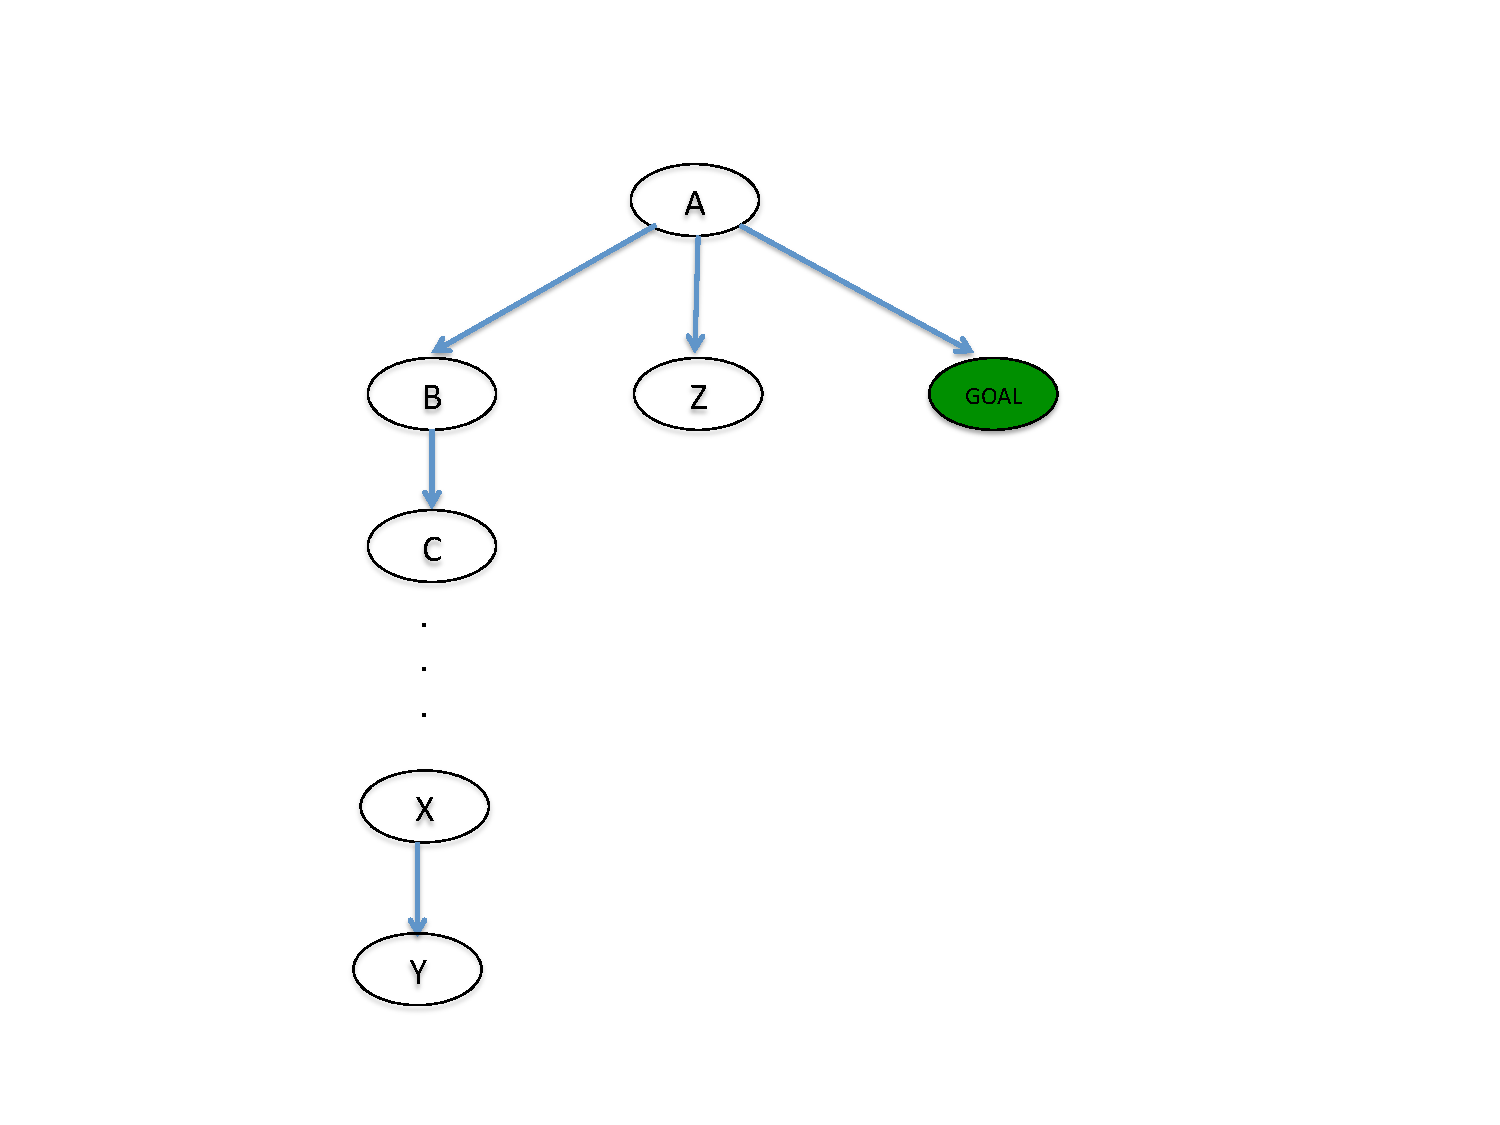
\includegraphics[scale=0.3]{dfs.pdf}
\caption{Example of graph where path-checking depth-first search takes more run time (explore 27 nodes A,B,...Z and goal) compared to breadth-first search takes (explore 4 nodes A,B,Z and Goal). }
\label{Figure 2}
\end{figure}

\begin{lstlisting}[language=java,caption={Output for path-checking DFS for start state of (3, 3, 1)}]
dfs path checking path length: 11 [(3, 1, 0), (3, 2, 1), (3, 0, 0), (3, 1, 1), (1, 1, 0), (2, 2, 1), (0, 2, 0), (0, 3, 1), (0, 1, 0), (0, 2, 1), (0, 0, 0)]
Nodes explored during last search:  13
Maximum memory usage during last search 12
\end{lstlisting}

\begin{lstlisting}[language=java,caption={Output for path-checking DFS for start state of (8, 5, 1)}]
dfs path checking path length: 33 
Nodes explored during last search:  40
Maximum memory usage during last search 34
\end{lstlisting}

Note that path-checking DFS saves significant memory compared to BFS. The maximum memory usage for the second case of start state (8,5,1) for path-checking DFS is 34 nodes while BFS requires memory usage of 62 nodes. This is because path-checking DFS only stores the node along the path (without a loop), and is thus the memory usage is restricted to the longest path while for BFS, the worse case space requirement will be to store all the nodes. However, the trade-off is that path-checking DFS might result in a longer run-time when a long, unsuccessful path is being explored. BFS avoids this problem by checking in increasing order of depth. An example of a graph in which path-checking DFS will take a much longer run time than BFS is given in Figure 2.\\

\section{Iterative deepening search}

We can perform iterative deepening search by implementing path-checking depth-first search in increasing order of depth until we discover the goal state. The implementation is given in Listing 13:\\

\begin{lstlisting}[language=java,caption={Iterative deepening search}]
public List<UUSearchNode> IDSearch(int maxDepth) {
	for(int i = 0; i < maxDepth; i++){
		HashSet<UUSearchNode> currentPath = new HashSet<>();
		currentPath.add(startNode);
		List<UUSearchNode> attempt = dfsrpc(startNode, currentPath, 0, i);
		if(attempt != null)
			return attempt;
	}
	return null;
}
\end{lstlisting}

The basic idea is that by performing path-checking DFS in increasing order of depth, we will be able to discover the shortest path to the goal state while ensuring that the upper bound for memory is the length of the shortest path to the goal state. \\

Listing 14 shows the output of iterative deepening search using path-checking DFS for start state of (8,5,1). It can be seen that the method is a lot more memory efficient than BFS. However, the trade-off is that the run-time is a lot longer since all the work that is used in the previous path-checking is thrown away with each new iteration of search.\\

Listing 15 shows the output of iterative deepening search using memomizing DFS for start state of (8,5,1). However, iterative deepening search using memomizing has the same space requirement as breadth-first search while the run time is often a lot longer. Therefore, it does not make sense to use memomizing DFS for iterative deepening search since it does not offer any advantage in terms of memory while the run time is longer than BFS. Instead, I will prefer to use path-checking DFS for iterative deepening search since it confers the advantage of being more efficient in terms of memory requirement even if it is at the expense of  a longer runtime.

\begin{lstlisting}[language=java,caption={Iterative deepening search using path-checking DFS for start state of (8,5,1)}]
Iterative deepening (path checking) path length: 23 
Nodes explored during last search:  19425295
Maximum memory usage during last search 24
\end{lstlisting}

\begin{lstlisting}[language=java,caption={Iterative deepening search using memomizing DFS for start state of (8,5,1)}]
Iterative deepening (memomizing) path length: 23 
Nodes explored during last search:  1398770
Maximum memory usage during last search 60
\end{lstlisting}

\section{Lossy missionaries and cannibals}

In the case where no more than $E$ missionaries could be eaten, we have to revise our state to include the number of cannibals and missionaries on both sides of the river i.e. $(m_1,c_1,m_2,c_2,b)$, where $m_1$ denotes number of missionaries at the start bank, $c_1$ denotes number of cannibals at the start bank, $m_2$ denotes number of missionaries at the finish bank, $c_2$ denotes number of cannibals at the finish bank, and $b$ denotes the number of boats at the start bank. We also have to change the original safe state condition to reflect the fact that $T_m$ (total number of missionaries) and $T_c$ (total number of cannibals) are no longer constants. The code is given below (in which I assume that whenever the number of cannibals exceeds the number of missionaries at either side, all the missionaries at that side will be eaten).

\begin{lstlisting}[language=java,caption={modified isSafeState and getSuccessors}]
boolean isSafeState(m_1,m_2,T_m,E){
	return m1+m2 >= T_m - E;
}
ArrayList<UUSearchNode> getSuccessors(m_1,m_2,c_1,c_2,b) {
	 ...
	if(b == 1) { // move away from start bank
		numMissionaries1 = m_1 - moveMissionaries;
		numCannibals1 = c_1 - moveCannibals;
		numMissionaries2 = m_2 + moveMissionaries;
		numCannibals2 = c_2 + moveCannibals;
		nextb = 0;
	}else{ 	/* same concept as above	*/ }		// move towards the finish bank
		
	if(numCannibals1 > numMissionaries1) numMissionaries1 = 0; // assumption
	if(numCannibals2 > numMissionaries2) numMissionaries2 = 0; // assumption
	CannibalNode potentialSuccessor = new CannibalNode(numMissionaries1,numCannibals1,numMissionaries2,numCannibals2,nextb,depth);
	if(moveCannibals+moveMissionaries != 0 && potentialSuccessor.isLegalState()
		&& potentialSuccessor.isSafeState()){
			array.add(potentialSuccessor);
	}
	...
	return array;
}
\end{lstlisting}

A very loose upperbound for the number of possible states can be estimated in the same manner described in the first section i.e. $S = (T_m+1)^2 \times (T_c+1)^2 \times (T_b+1)^2$ since the state can be represented by  $(m_1,c_1,m_2,c_2,b)$ and $0\le m_1 \le T_m$,  $0\le c_1 \le T_c$,  $0\le m_2 \le T_m$,  $0\le c_2 \le T_c$,  $0\le b \le T_b$.

\section{Additional Features}

My code considers the case of different boat size (so instead of carrying a maximum of 2 people, the boat can carry a maximum of any number of people). I also implemented the Lossy missionaries and cannibals problem and an optional description of the implementation and results is in the Appendix.

\section{Appendix (Optional features)}
\subsection{Varying boat size}

Because of the way I implement the \verb`getSuccessors` method, my code is flexible enough to allow for varying boat size. For the start state of $(8,5,1)$, I change the variable $BOAT\_SIZE$ in CannibalProblem.java and tried $BOAT\_SIZE = 3, 6, 9, 13$. The output for BFS is presented below:\\

\begin{lstlisting}[language=java,caption={BFS for start state of (8,5,1) and BOAT\_SIZE = 3}]
bfs path length:  11 [(8, 2, 0), (8, 3, 1), (5, 3, 0), (5, 4, 1), (4, 2, 0), (4, 3, 1), (3, 1, 0), (3, 2, 1), (2, 0, 0), (2, 1, 1), (0, 0, 0)]
Nodes explored during last search:  62
Maximum memory usage during last search 62
\end{lstlisting}

\begin{lstlisting}[language=java,caption={BFS for start state of (8,5,1) and BOAT\_SIZE = 6}]
bfs path length:  5 [(8, 2, 0), (8, 3, 1), (4, 1, 0), (4, 2, 1), (0, 0, 0)]
Nodes explored during last search:  64
Maximum memory usage during last search 64
\end{lstlisting}

\begin{lstlisting}[language=java,caption={BFS for start state of (8,5,1) and BOAT\_SIZE = 9}]
bfs path length:  3 [(8, 0, 0), (8, 1, 1), (0, 0, 0)]
Nodes explored during last search:  64
Maximum memory usage during last search 64
\end{lstlisting}

\begin{lstlisting}[language=java,caption={BFS for start state of (8,5,1) and BOAT\_SIZE = 13}]
bfs path length:  1 [(0, 0, 0)]
Nodes explored during last search:  64
Maximum memory usage during last search 64
\end{lstlisting}

Note that the path length of the shortest path decreases with an increase in $BOAT\_SIZE$. This is because the successors for the problem with a smaller $BOAT\_SIZE$ will also be the successors for the problem with a larger $BOAT\_SIZE$ (the reverse is not true) and therefore there are more possibilities or nodes to explore at each stage with a larger $BOAT\_SIZE$. Note that in the case where the $BOAT\_SIZE = T_c + T_m = 8 + 5 =13$, the path length is 1 since the shortest path will be for all the missionaries and all the cannibals to cross the river at once, which makes logical sense.

\subsection{Implementation of Lossy missionaries and cannibals}

I also implemented the lossy missionaries and cannibals problem as described in section 7. I made the assumption that whenever the number of cannibals exceeds the number of missionaries at either side, all the missionaries at that side will be eaten. To run and test the code, simply refer to the instructions in the README.\\

To check for the correctness of my solution, I implemented the Lossy method with the degree of ``lossness'' $E = 0$. I will expect to get the same result as the original algorithm, and I did. The output for the lossy method is given in Listing 21, for start state $(8,5,0,0,1)$ and goal state $(0,0,8,5,0)$ (recall the notation $(m_1,c_1,m_2,c_2,b)$. \\

\begin{lstlisting}[language=java,caption={Output for lossy algorithm for start state of (8,5,0,0,1) and E = 0}]
====================
Lossy Implementation
Lossy bfs path length:  23 [(8, 3, 0, 2, 0), (8, 4, 0, 1, 1), (8, 2, 0, 3, 0), (8, 3, 0, 2, 1), (6, 3, 2, 2, 0), (6, 4, 2, 1, 1), (5, 3, 3, 2, 0), (5, 4, 3, 1, 1), (5, 2, 3, 3, 0), (5, 3, 3, 2, 1), (4, 2, 4, 3, 0), (4, 3, 4, 2, 1), (4, 1, 4, 4, 0), (4, 2, 4, 3, 1), (3, 1, 5, 4, 0), (3, 2, 5, 3, 1), (3, 0, 5, 5, 0), (3, 1, 5, 4, 1), (2, 0, 6, 5, 0), (2, 1, 6, 4, 1), (1, 0, 7, 5, 0), (1, 1, 7, 4, 1), (0, 0, 8, 5, 0)]
Nodes explored during last search:  62
Maximum memory usage during last search 62
--------
Lossy dfs memoizing path length: 33 [(8, 3, 0, 2, 0), (8, 4, 0, 1, 1), (8, 2, 0, 3, 0), (8, 3, 0, 2, 1), (6, 3, 2, 2, 0), (6, 4, 2, 1, 1), (5, 4, 3, 1, 0), (5, 5, 3, 0, 1), (5, 3, 3, 2, 0), (5, 4, 3, 1, 1), (5, 2, 3, 3, 0), (5, 3, 3, 2, 1), (4, 3, 4, 2, 0), (4, 4, 4, 1, 1), (4, 2, 4, 3, 0), (4, 3, 4, 2, 1), (4, 1, 4, 4, 0), (4, 2, 4, 3, 1), (3, 2, 5, 3, 0), (3, 3, 5, 2, 1), (3, 1, 5, 4, 0), (3, 2, 5, 3, 1), (3, 0, 5, 5, 0), (3, 1, 5, 4, 1), (2, 1, 6, 4, 0), (2, 2, 6, 3, 1), (2, 0, 6, 5, 0), (2, 1, 6, 4, 1), (1, 0, 7, 5, 0), (1, 1, 7, 4, 1), (0, 1, 8, 4, 0), (0, 2, 8, 3, 1), (0, 0, 8, 5, 0)]
Nodes explored during last search:  40
Maximum memory usage during last search 40
--------
Lossy dfs path checking path length: 33 [(8, 3, 0, 2, 0), (8, 4, 0, 1, 1), (8, 2, 0, 3, 0), (8, 3, 0, 2, 1), (6, 3, 2, 2, 0), (6, 4, 2, 1, 1), (5, 4, 3, 1, 0), (5, 5, 3, 0, 1), (5, 3, 3, 2, 0), (5, 4, 3, 1, 1), (5, 2, 3, 3, 0), (5, 3, 3, 2, 1), (4, 3, 4, 2, 0), (4, 4, 4, 1, 1), (4, 2, 4, 3, 0), (4, 3, 4, 2, 1), (4, 1, 4, 4, 0), (4, 2, 4, 3, 1), (3, 2, 5, 3, 0), (3, 3, 5, 2, 1), (3, 1, 5, 4, 0), (3, 2, 5, 3, 1), (3, 0, 5, 5, 0), (3, 1, 5, 4, 1), (2, 1, 6, 4, 0), (2, 2, 6, 3, 1), (2, 0, 6, 5, 0), (2, 1, 6, 4, 1), (1, 0, 7, 5, 0), (1, 1, 7, 4, 1), (0, 1, 8, 4, 0), (0, 2, 8, 3, 1), (0, 0, 8, 5, 0)]
Nodes explored during last search:  40
Maximum memory usage during last search 34
--------
Lossy Iterative deepening (path checking) path length: 23 [(8, 3, 0, 2, 0), (8, 4, 0, 1, 1), (8, 2, 0, 3, 0), (8, 3, 0, 2, 1), (6, 3, 2, 2, 0), (6, 4, 2, 1, 1), (5, 3, 3, 2, 0), (5, 4, 3, 1, 1), (5, 2, 3, 3, 0), (5, 3, 3, 2, 1), (4, 2, 4, 3, 0), (4, 3, 4, 2, 1), (4, 1, 4, 4, 0), (4, 2, 4, 3, 1), (3, 1, 5, 4, 0), (3, 2, 5, 3, 1), (3, 0, 5, 5, 0), (3, 1, 5, 4, 1), (2, 0, 6, 5, 0), (2, 1, 6, 4, 1), (1, 0, 7, 5, 0), (1, 1, 7, 4, 1), (0, 0, 8, 5, 0)]
Nodes explored during last search:  19425295
Maximum memory usage during last search 24
\end{lstlisting}

I try to think of a case in which lossy implementation will give a different result from the original implementation (i.e. either the original problem is unsolvable and can now be solved using the lossy method, or there is shorter path if we allow for a few sacrifices). However, I am unable to think of a situation as the time of writing this report.\\


\end{document}